\documentclass[12pt]{article}
\usepackage[document]{ragged2e}
\usepackage[section]{placeins}
\usepackage{graphicx}
\graphicspath{ {./images/} }

\title{Jelgenerátor, négyszög és háromszög jel generálása}
\author{Mészáros Adél}

\begin{document}
  \maketitle
  \newpage

  \section{Terv specifikálása}
    A laborgyakorlat célja egy olyan áramkör megvalósítása FPGA segítségével, amely képes háromszög és négyszög jelek generálására. A felhasználó kiválaszthatja,
    hogy milyen tipusú jelet szeretne generálni és állithatja annak amplitudóját és frekvenciáját.
    \newline
    A hardvert két fő komponens alkotja: 
    \begin{enumerate}
      \item Digitál-analóg konverter
      \item FPGA-n megvalósított vezérlő áramkör
    \end{enumerate}

    \subsection{Digitál-analóg konverter}
      Az AD5302/AD5312/AD5322 tipusú digitál-analóg tipusó konvertert fogom használni.

      \begin{figure}[h]
        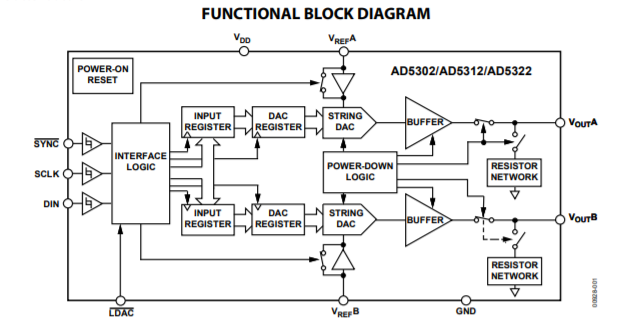
\includegraphics{dac_kapcs}
        \centering
        \caption{A digitál-analóg konverter kapcsolási ra}
      \end{figure}

    \begin{figure}[h]
      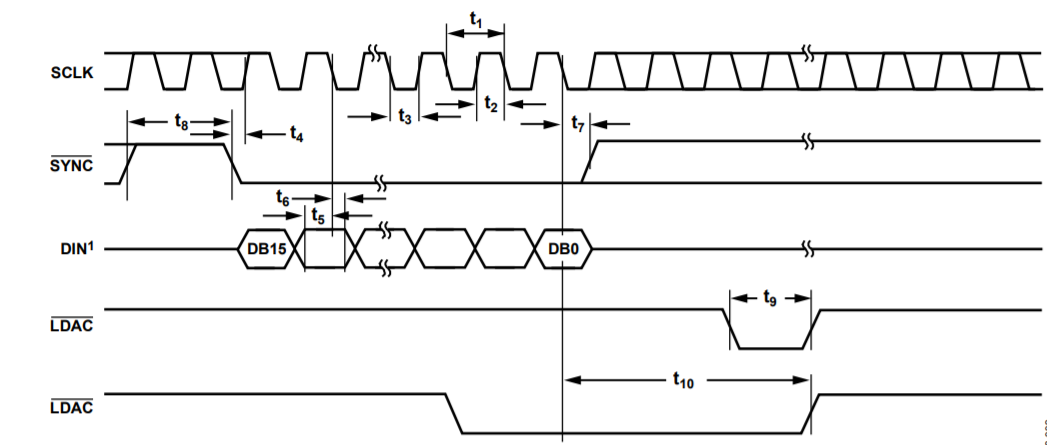
\includegraphics[width=\textwidth,height=\textheight,keepaspectratio]{dac_jelek}
      \centering 
      \caption{A jelek változásai} 
    \end{figure}
    \newpage
    \begin{itemize}
      \item \textbf{LDAC} \linebreak
            \quad 0 - kimenet frissítése \linebreak
            \quad 1 - kimeneti érték változatlan
      \item \textbf{SYNC} \linebreak
            \quad 0 - bemeneti regiszter feltöltésének kezdése \linebreak
            \quad 1 - ha a bemeneti regiszter nem volt feltöltve, a feltöltés megszakad
      \item \textbf{SCLK} \linebreak
            \quad A bemeneti regiszter feltöltését ütemező órajel. Minden lemenő élre újabb bit töltődik be.  
      \item \textbf{DIN} \linebreak
            \quad A regiszterbe töltött bit értéke
    \end{itemize}

    \newpage
    \begin{figure}[h]
      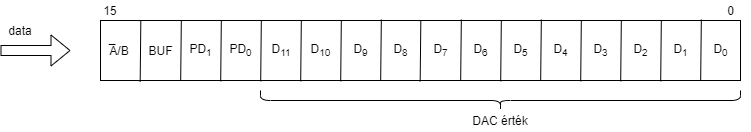
\includegraphics[width=\textwidth,height=\textheight,keepaspectratio]{bitek}
      \centering  
      \caption{A 16 bit felosztása}
    \end{figure}

    \begin{itemize}
      \item \textbf{PDo, PD1} \linebreak
            \quad Power-down mode, ha mindkettő '0', normál üzemmód, máskülönben energiatakarékos üzemmód.
      \item \textbf{BUF} \linebreak
            \quad a reference buffer, ha '0', az ADC, 0-tól Vref-ig üzemel, ha '1' az ADC 1-től Vref-ig üzemel.
      \item \textbf{A/B} \linebreak
            \quad 0 - az A kimenetet (használja) updateolja \linebreak
            \quad 1 - a B kimenetet (használja) updateolja
    \end{itemize}
    \[V_{out}=(V_{ref}*D)/2^{12}\]
    
    \paragraph{Időzítések}
    \begin{itemize}
        \item [--]\textbf{SCLK} periódus, minimum 33 ns
        \item [--]\textbf{DIN} minimum 5 ns-el az órajel lemenő éle előtt és az órajel lemenő éle után
        \item [--]\textbf{SYNC} minimum 100 ns 'high', az olvasások között. Az órajel felmenő éle előtt (vagy azzal egyszerre) kell lehúzni, hogy elkedjük az olvasást
        \item [--]\textbf{LDAC} minimum 20 ns az adatok betöltéséhez.
        \item [--]\textbf{SCLK} periódus, minimum 33 ns 
    \end{itemize}
   
    
    \paragraph{Vezérlés\newline}{
  Feltöltöm a bemeneti regisztert az 'adat' értékével és lezárom az írási ciklust.
  Ha az A kimenetet szeretnénk hasznlni, az 'adat' változó első 4 bitje '0', a következő 12 pedig az értéket fogja tartalmazni.\newpage}
  \newpage 
  \subsection{FPGA modulok\newline}
  \paragraph{}
  Négy nagy modult különböztetünk meg. A bemeneti modult, itt megadja a felhasználó a kívánt jel tipusát, frekvenciáját és amplitudóját.
  Négyszög és háromszüg jelet előállító modulokat, amelyek generálják a megfelelő frekvenciában és amplitudóban a kommunikációs modulnak a biteket.
  A kommunikációs modul továbbítja a jeleket a digitál-analóg konverternek.
      \begin{figure}[hb]
        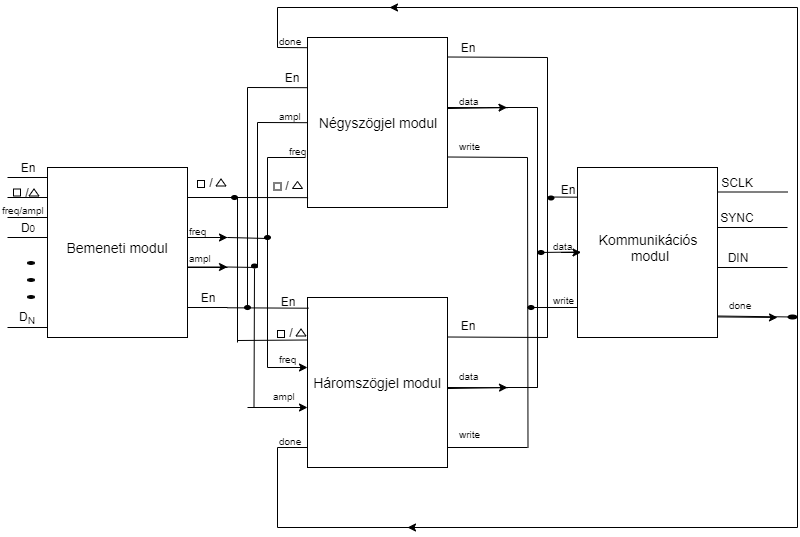
\includegraphics[width=\textwidth]{modulok}
        \centering  
        \caption{Modulok és a köztük lévő kapcsolat}
      \end{figure}

      
      


\end{document}
